\chapter{Sự tạo ảnh bởi thấu kính}


\section{Lý thuyết trọng tâm}

\subsection{Khái niệm ảnh và vật trong quang học}
\begin{center}
	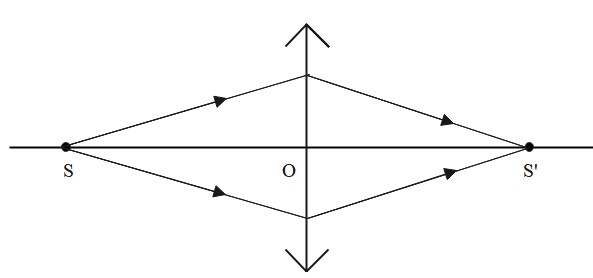
\includegraphics[scale=0.7]{../figs/VN11-PH-38-L-026-2-h1.jpg}
\end{center}

Ảnh điểm là điểm đồng quy của chùm tia ló hay đường kéo dài của chúng.
Một ảnh điểm là:
\begin{itemize}
	\item thật nếu chùm tia ló là chùm hội tụ.
	\item ảo nếu chùm tia ló là chùm phân kỳ.
	\end{itemize}

Vật điểm là điểm đồng quy của chùm tia tới hay đường kéo dài của chúng.
Một vật điểm là:
\begin{itemize}
	\item thật nếu chùm tia tới là chùm phân kỳ.
	\item ảo nếu là chùm tia tới là chùm hội tụ. 
\end{itemize}
\subsection{ Đường truyền của tia sáng qua thấu  kính}
\subsubsection{ Đường truyền của tia sáng qua  thấu kính hội tụ}
\begin{itemize}
	\item Tia tới đi qua quang tâm O thì cho tia ló tiếp tục truyền thẳng.
	\begin{center}
		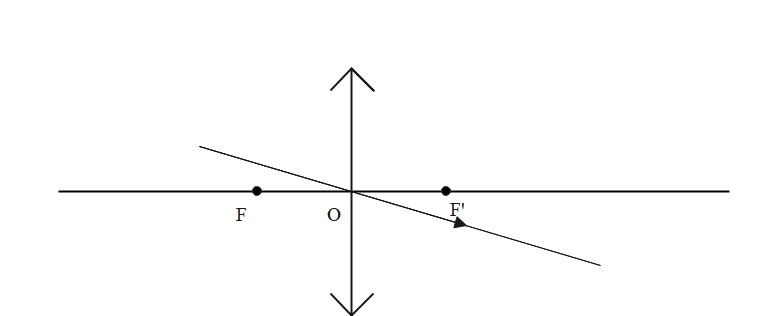
\includegraphics[scale=0.7]{../figs/VN11-PH-38-L-026-2-h19.jpg}
	\end{center}
	\item Tia tới song song trục chính thì cho tia ló qua tiêu điểm ảnh chính F'.
		\begin{center}
		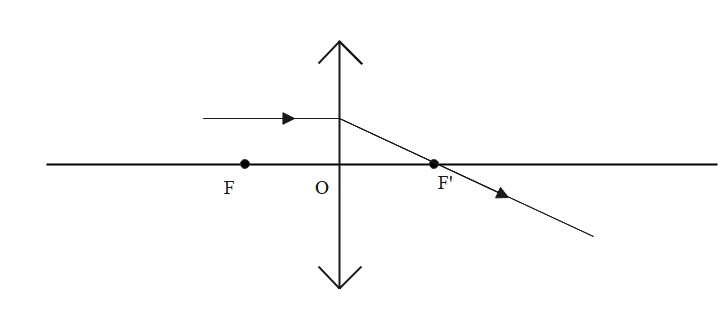
\includegraphics[scale=0.7]{../figs/VN11-PH-38-L-026-2-h20.jpg}
	\end{center}
	 \item Tia tới đi qua tiêu điểm vật chính F thì cho tia ló song song trục chính. 
	 	\begin{center}
	 	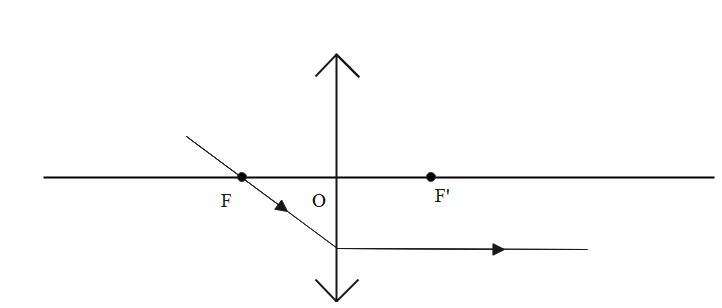
\includegraphics[scale=0.7]{../figs/VN11-PH-38-L-026-2-h21.jpg}
	 \end{center}
\end{itemize}

\subsubsection{ Đường truyền của tia sáng qua thấu  kính thấu kính phân kỳ}
\begin{itemize}
\item Tia tới đi qua quang tâm O thì cho tia ló tiếp tục truyền thẳng.
	\begin{center}
	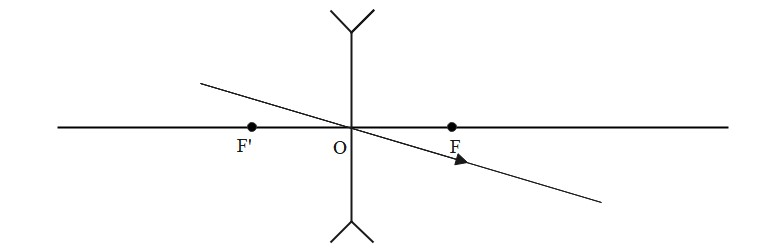
\includegraphics[scale=0.7]{../figs/VN11-PH-38-L-026-2-h22.jpg}
\end{center}
\item Tia tới song song trục chính thì cho tia ló có đường kéo dài qua tiêu điểm ảnh chính F'.
	\begin{center}
	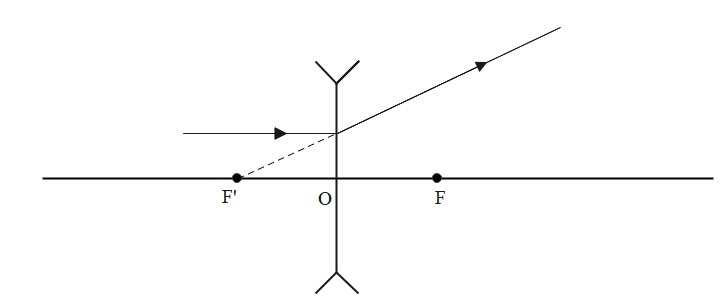
\includegraphics[scale=0.7]{../figs/VN11-PH-38-L-026-2-h23.jpg}
\end{center}
\item Tia tới có đường kéo dài đi qua tiêu điểm vật chính F thì cho tia ló song song trục chính.
	\begin{center}
	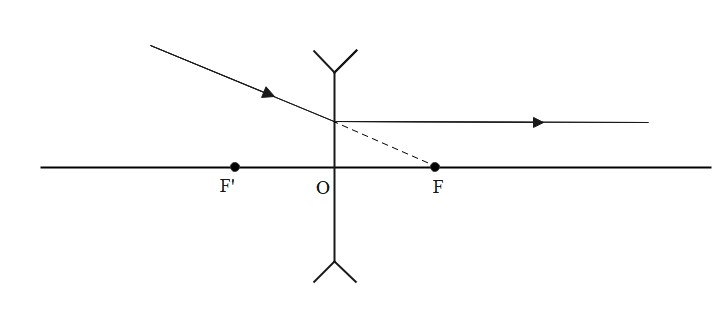
\includegraphics[scale=0.7]{../figs/VN11-PH-38-L-026-2-h24.jpg}
\end{center} 
\end{itemize}
\subsection{Cách dựng ảnh tạo bởi thấu kính}
Sử dụng 2 trong số các tia tới đặc biệt sau:
\begin{itemize}
	\item Tia tới qua quang tâm O thì tia ló tiếp tục truyền thẳng.
	\item Tia tới song song với trục chính của thấu kính. thì tia ló (hoặc đường kéo dài của tia ló) sẽ đi qua tiêu điểm ảnh chính.
	\item Tia tới qua tiêu điểm vật chính F (hay có đường kéo dài qua F) thì tia ló sẽ song song với trục chính.
\end{itemize}
\begin{center}
	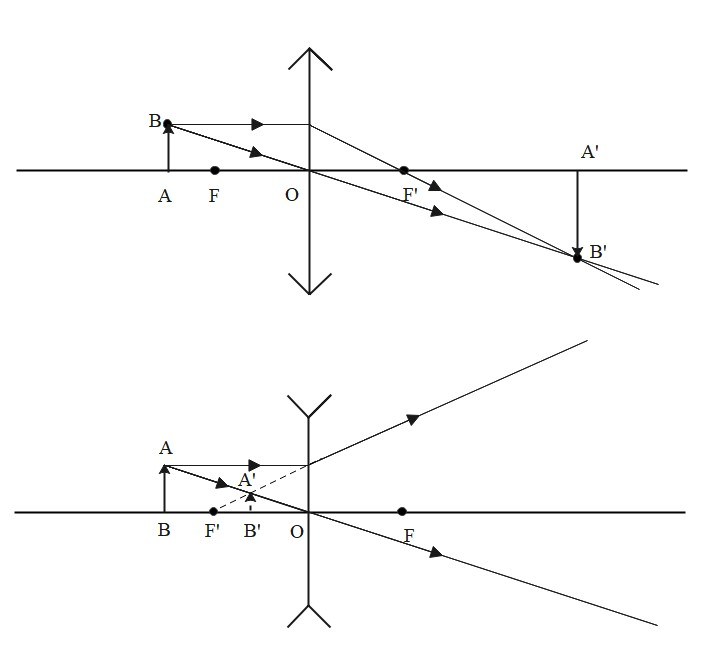
\includegraphics[scale=0.7]{../figs/VN11-PH-38-L-026-2-h25.jpg}
\end{center}
 Giao điểm của các tia ló chính là vị trí ảnh. 

Trường hợp tia sáng bất kỳ thì cách xác định tia ló như sau:
\begin{itemize}
	\item Dựng trục phụ song song với tia tới.
	\item Từ F' dựng đường thẳng vuông góc  với trục chính , cắt trục phụ tại $\text{F'}_1$.
	\item Nối điểm tới I và $\text{F'}_1$ ta được tia ló.
	\begin{center}
		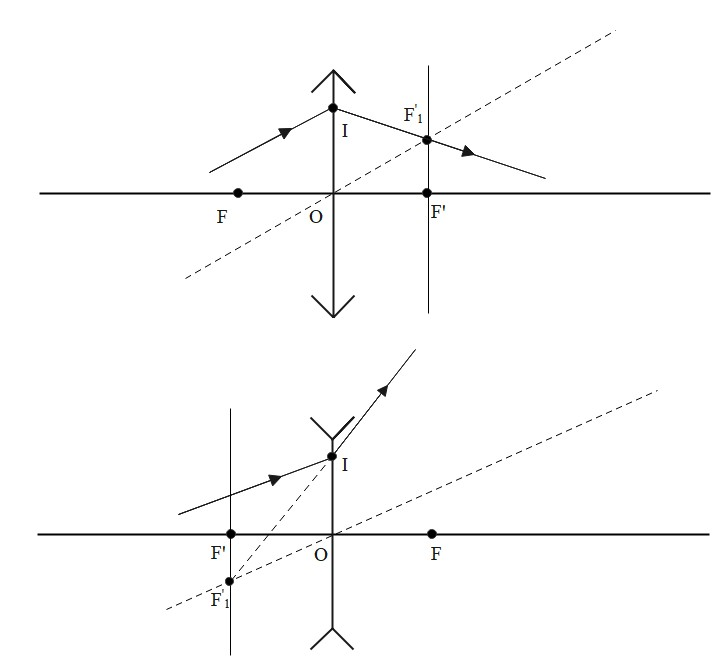
\includegraphics[scale=0.7]{../figs/VN11-PH-38-L-026-2-h26.jpg}
	\end{center} 
\end{itemize}

\subsection{ Các trường hợp ảnh tạo bởi thấu kính}
Ảnh của một vật tạo bởi thấu kính có những đặc điểm xác định về tính chất (thật, ảo), chiều và độ lớn.

\textbf{Với thấu kính hội tụ:}

Nếu vật thật cho \textit{ảnh thật}:
\begin{itemize}
	\item Ảnh ngược chiều vật (hứng được trên màn).
	\item Ảnh có kích thước: 
\begin{itemize}
	\item nhỏ hơn vật vật nếu $d>2f$,
	\item lớn hơn vật nếu $d<f<2f$,
	\item bằng vật nếu $d=2f$.
\end{itemize}
\end{itemize}

Nếu vật thật cho \textit{ảnh ảo}: ảnh ảo luôn cùng chiều vật và lớn hơn vật.

\textbf{Với thấu kính phân kỳ}:

Vật thật luôn cho ảnh ảo, cùng chiều vật và nhỏ hơn vật. 
\subsection{Các công thức về thấu kính}
\subsubsection{Công thức xác định vị trí ảnh}
\begin{equation}
\dfrac{1}{f}=\dfrac{1}{d}+\dfrac{1}{d'},
\end{equation}
trong đó:
\begin{itemize}
	\item $f$ là tiêu cự của thấu kính;
	\item $d$ là khoảng cách từ vật đến thấu kính;
	\item $d'$ là khoảng cách từ ảnh đến thấu kính. 
\end{itemize}
Quy ước: 
\begin{itemize}
	\item vật thật: $d>0$;
	\item vật ảo: $d<0$;
	\item ảnh thật: $d>0$;
	\item ảnh ảo: $d<0$;
\end{itemize}
\subsubsection{Công thức xác định số phóng đại ảnh}
\begin{equation}
k=-\dfrac{d'}{d}=\dfrac{f}{f-d}=\dfrac{f-d'}{f},
\end{equation}
trong đó:
\begin{itemize}
	\item $k$ là số phóng đại của ảnh;
	\item $f$ là tiêu cự của thấu kính;
	\item $d$ là khoảng cách từ vật đến thấu kính;
	\item $d'$ là khoảng cách từ ảnh đến thấu kính. 
\end{itemize}


\section{Bài tập }
\begin{dang}{Đường truyền của tia sáng qua thấu  kính thấu kính}
\end{dang}

 \viduii{1}{

 Chọn phát biểu \textbf{không đúng}
\begin{mcq}
	\item Tia tới đi qua quang tâm O thì cho tia ló tiếp tục truyền thẳng.
	\item Tia tới song song với trục chính của thấu kính. thì tia ló (hoặc đường kéo dài của tia ló) sẽ đi qua tiêu điểm vật chính.
	\item  Tia tới qua tiêu điểm vật chính F (hay có đường kéo dài qua F) thì tia ló sẽ song song với trục chính.
	\item Tia tới song song với trục chính của thấu kính. thì tia ló (hoặc đường kéo dài của tia ló) sẽ đi qua tiêu điểm ảnh chính.
\end{mcq}}
{

\begin{center}
	\textbf{Hướng dẫn giải:}
\end{center}

{Tia tới song song với trục chính của thấu kính. thì tia ló (hoặc đường kéo dài của tia ló) sẽ đi qua tiêu điểm ảnh chính.
	
\textbf{	Đáp án: B.}
}
}
\viduii{1}{
Để vẽ tia ló trong trường hợp tia sáng bất kỳ tới thấu kính thì phải vẽ thêm 
\begin{mcq}
	\item tiêu điểm vật chính. 
	\item tiêu điểm ảnh chính. 
	\item trục phụ.
	\item quang tâm O.
\end{mcq}}
{
\begin{center}
	\textbf{Hướng dẫn giải:}
\end{center}
{Để vẽ tia ló trong trường hợp tia sáng bất kỳ tới thấu kính thì phải vẽ thêm trục phụ. 
	
		\textbf{Đáp án: C.}
}}
\begin{dang}{Sự tạo ảnh bới thấu kính}
\end{dang}
\viduii{1}{
Đối với thấu kính hội tụ thì
\begin{mcq}
	\item vật thật luôn cho ảnh ảo.
	\item vật thật có thể cho ảnh thật hoặc ảnh ảo.
	\item vật thật luôn cho ảnh thật.
	\item  vật thật luôn cho ảnh ảo, nhỏ hơn vật. 
\end{mcq}}
{
\begin{center}
	\textbf{Hướng dẫn giải:}
\end{center}

{ Đối với thấu kính hội tụ thì vật thật có thể cho ảnh thật hoặc ảnh ảo.
		
	\textbf{Đáp án: B.}
}
}
\viduii{1}{
Đặt một vật AB trước một thấu kính. Sau thấu kính này ta đặt một màn ảnh và hứng được ảnh. Đó là
\begin{mcq}
	\item ảnh thật, thấu kính là thấu kính phân kỳ.
	\item ảnh thật, thấu kính là thấu kính hội tụ.
	\item ảnh ảo, thấu kính là thấu kính phân kỳ.
	\item  ảnh ảo, thấu kính là thấu kính hội tụ.
\end{mcq}}{
\begin{center}
	\textbf{Hướng dẫn giải:}
\end{center}


{ Ảnh hứng được trên màn chắn phải là ảnh thật. Trong chương trình, ta đã học rằng chỉ có thấu kính hội tụ mới cho ảnh thật.
\textbf{	Đáp án: B.}
}}

\viduii{1}{
Đối với thấu kính phân kì, nhận xét nào sau đây về tính chất ảnh của một vật thật là đúng?
\begin{mcq}
	\item Vật thật luôn cho ảnh ảo, ngược chiều và lớn hơn vật.
	\item Vật thật luôn cho ảnh thật, ngược chiều, nhỏ hơn vật.
	\item Vật thật luôn cho ảnh ảo, cùng chiều và nhỏ hơn vật.
	\item Vật thật có thể cho ảnh thật, ngược chiều và lớn hơn hay nhỏ hơn vật hoặc ảnh ảo, cùng chiều và lớn hơn vật.
\end{mcq}}{
\begin{center}
	\textbf{Hướng dẫn giải:}
\end{center}



{ Đối với thấu kính phân kì, vật thật luôn cho ảnh ảo, cùng chiều và nhỏ hơn vật.
	\textbf{Đáp án: C.}
}
}
\viduii{4}{
Ảnh thu được từ thấu kính hội tụ của vật thật là
\begin{mcq}
	\item ảnh thật luôn lớn hơn vật.
	\item ảnh ảo luôn nhỏ hơn vật.
	\item ảnh thật lớn hơn vật, nhỏ hơn vật hoặc cao bằng vật còn phụ thuộc vào khoảng cách từ vật đến thấu kính.
	\item Ảnh ảo lớn hơn vật, nhỏ hơn vật hoặc cao bằng vật còn phụ thuộc vào độ cao của vật.
\end{mcq}}{
\begin{center}
	\textbf{Hướng dẫn giải:}
\end{center}


{ Ảnh thu được từ thấu kính hội tụ của vật thật là ảnh thật lớn hơn hoặc nhỏ hơn vật còn phụ thuộc vào khoảng cách từ vật đến thấu kính. 
	
Ta giả sử, $d$ là khoảng cách từ vật đến thấu kính, $f$ là tiêu cự của thấu kính.

Khi $f<d<2f$ thì ta thu được ảnh thật, ngược chiều, lớn hơn vật.

Khi $d=2f$ thì ta thu được ảnh thật, ngược chiều, cao bằng hơn vật.

Khi $d>2f$ thì ta thu được ảnh thật, ngược chiều, nhỏ hơn vật.

\textbf{	Đáp án: C.}
}
}
\viduii{1}{
 Ta thu được ảnh thật, ngược chiều và cùng kích thước như vật, khi
\begin{mcq}
	\item vật ở trước một thấu kính hội tụ có khoảng cách đến thấu kính lớn hơn tiêu cự của thấu kính chút ít.
	\item vật ở trước thấu kính hội tụ, khoảng cách tới thấu kính bằng hai lần tiêu cự.
	\item vật ở trong khoảng tiêu cự của thấu kính hội tụ.
	\item  vật tại tiêu điểm của thấu kính hội tụ.
\end{mcq}}{
\begin{center}
	\textbf{Hướng dẫn giải:}
\end{center}


{ Ta thu được ảnh thật, ngược chiều và cùng kích thước như vật, khi vật ở trước thấu kính hội tụ, khoảng cách tới thấu kính bằng hai lần tiêu cự.
	
	\textbf{Đáp án: B.}
}
}


